\section{Isochrone Fitting}\label{sec:isoFit}
We fit pairs of isochrones to the HUGS data for NGC 2808 using \fidanka, as
descrbed in \S {\color{red}FIDANKA SECTION}. Two isochrones, one for Population
A and one for Population E are fit simultaneously. These isochrones are
constrained to have distance modulus, $\mu$, and color excess, E(B-V) which
agree to within 1\%. Moreover, we constrain the mixing length, $\alpha_{ML}$, for any two isochrones in a set to be within 0.5 of one and other. For every isochrone in the
set of combination of which fulfilling these constraints $\mu$, $E(B-V)$,
Age$_{A}$, and $Age_{B}$ are optimized to reduce the $\chi^{2}$ distance
between the fiducial lines and the isochrones. Because we fit fiducial lines
directly, we do not need to consider the binary population fraction, $f_{bin}$,
as a free parameter.

The best fit isochrones are shown in Figure \ref{fig:BestFitResults} and optimized
parameters for these are presented in Table \ref{tab:BestFitResults}. We find helium mas fractions which are consistent with those identified in past literature \citep[e.g.][]{Milone2015}. Note that our helium mass fraction gird has a spacing of 0.03 between grid points and we are therefore unable to resolve between certain proposed helium mass fractions for the younger sequence (for example between 0.37 and 0.39).

\begin{figure*}
  \centering
  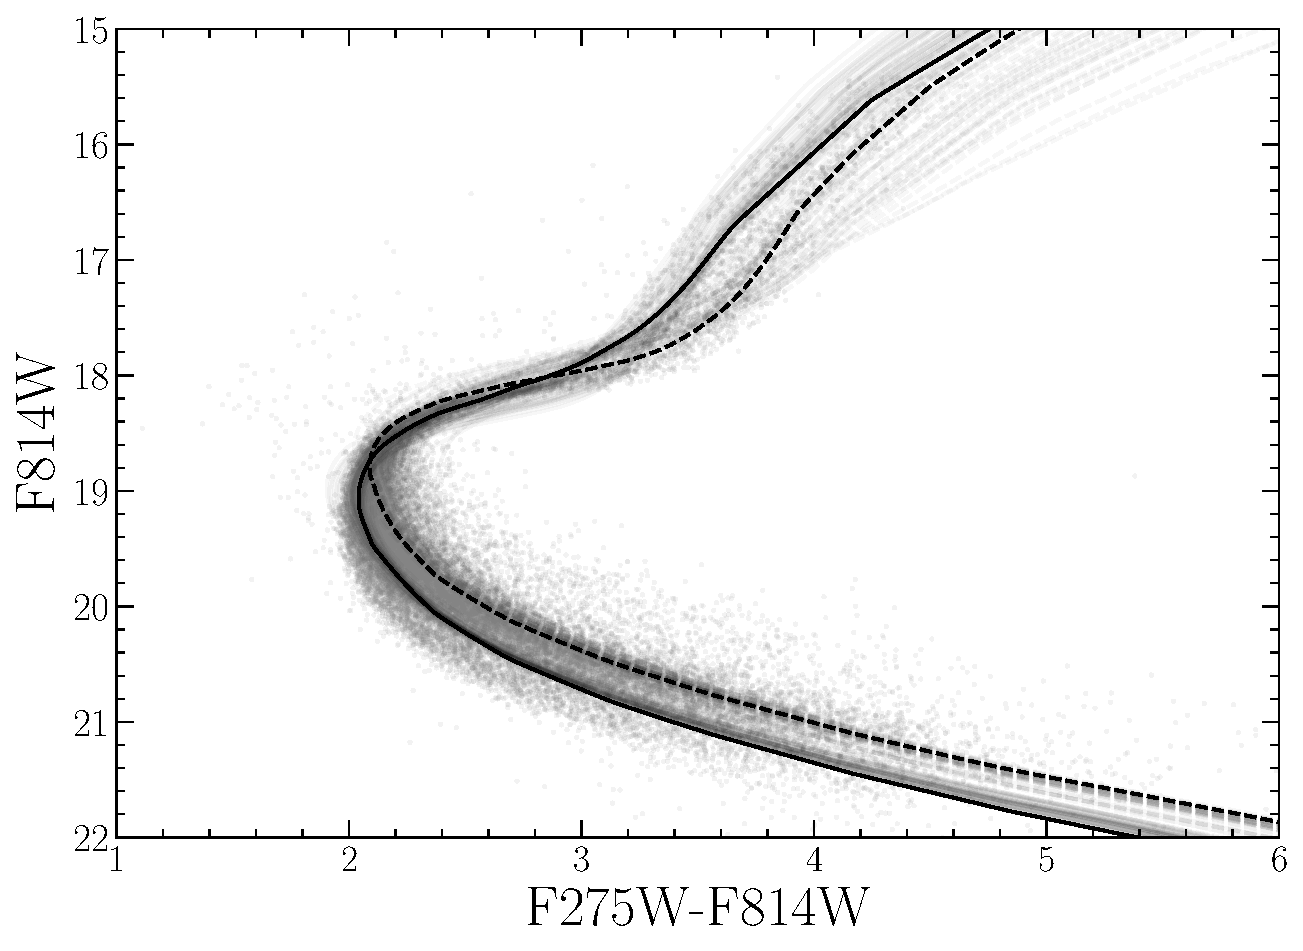
\includegraphics[width=0.9\textwidth]{src/figures/BestFitResults.pdf}
  \label{fig:BestFitResults}
  \caption{Best fit isochrone results for NGC 2808.}
\end{figure*}

\begin{table*}
  \centering
  \begin{tabular}{c | c c c c c c}
    \hline
    population & age & distance modulus & extinction & Y & $\alpha_{ML}$ & $\chi^{2}_{\nu}$\\
    & [Gyr] & & [mag] & & &\\
    \hline
    \hline
    A & 12.3 & 14.91 & 0.54 & 0.24 & 1.901 & 0.014\\
    E & 14.3 & 14.96 & 0.54 & 0.39 & 1.750 & 0.017 \\
    \hline
  \end{tabular}
  \label{tab:BestFitResults}
  \caption{Best fit parameters derived from fitting isochrones to the fiducual lines derived from the NCG 2808 photometry.}
\end{table*}


Past literature \citep[e.g. ][]{Milone2015, Milone2018} have found helium mass fraction variation from the low redmost to bluemost populations of $\sim 0.12$. Here we find a helium mass fraction variation of 0.15 which, given the spacing of the helium grid we use \textbf{is consistent with these past results}.

\subsection{The Number of Populartions in NGC 2808}
\fidanka provides a somewhat straigtforward way to estimate the number of populations expected in a given magnitude bin given the observations. See Section \ref{sec:fidanka} for specific implimentaiton details. Here we preform an analysis of the number of populations seen in the NGC 2808 F814W-F274W vs F814W color-magnitude diagram. We find that for the majority of the main sequence and red giant branches BGMM prefers two populations; wherease, near the main sequnce turn off and on the majority of the subgiant branches BGMM prefers a single population model.

{\color{red} Make Figure showing the BGMM fit predictions for each star vs. distance to pop mean line, does a good job of visualizing the predicted number of populations}


\subsection{ACS-HUGS Photometric Zero Point Offset}
The Hubble legacy archive photometry used in this work is calibrated to the
Vega magnitude system. However, we have found that the photometry has a
systematic offset of $\sim0.026$ magnitudes in the F814W band when
compared to the same stars in the ACS survey (Figure \ref{fig:offset}). The
exact cause of this offset is unknown, but it is likely due to a difference in
the photometric zero point between the two surveys. A full correction of this
offset would require a careful re-reduction of the HUGS photometry, which is
beyond the scope of this work. We instead recognize a 0.02 inherent uncertainty
in the inferred magnitude of any fit when comparing to the ACS survey. This
uncertainty is small when compared to the uncertainty in the
distance modulus and should not affect the conclusion of this
paper. 

\begin{figure*}
  \centering
  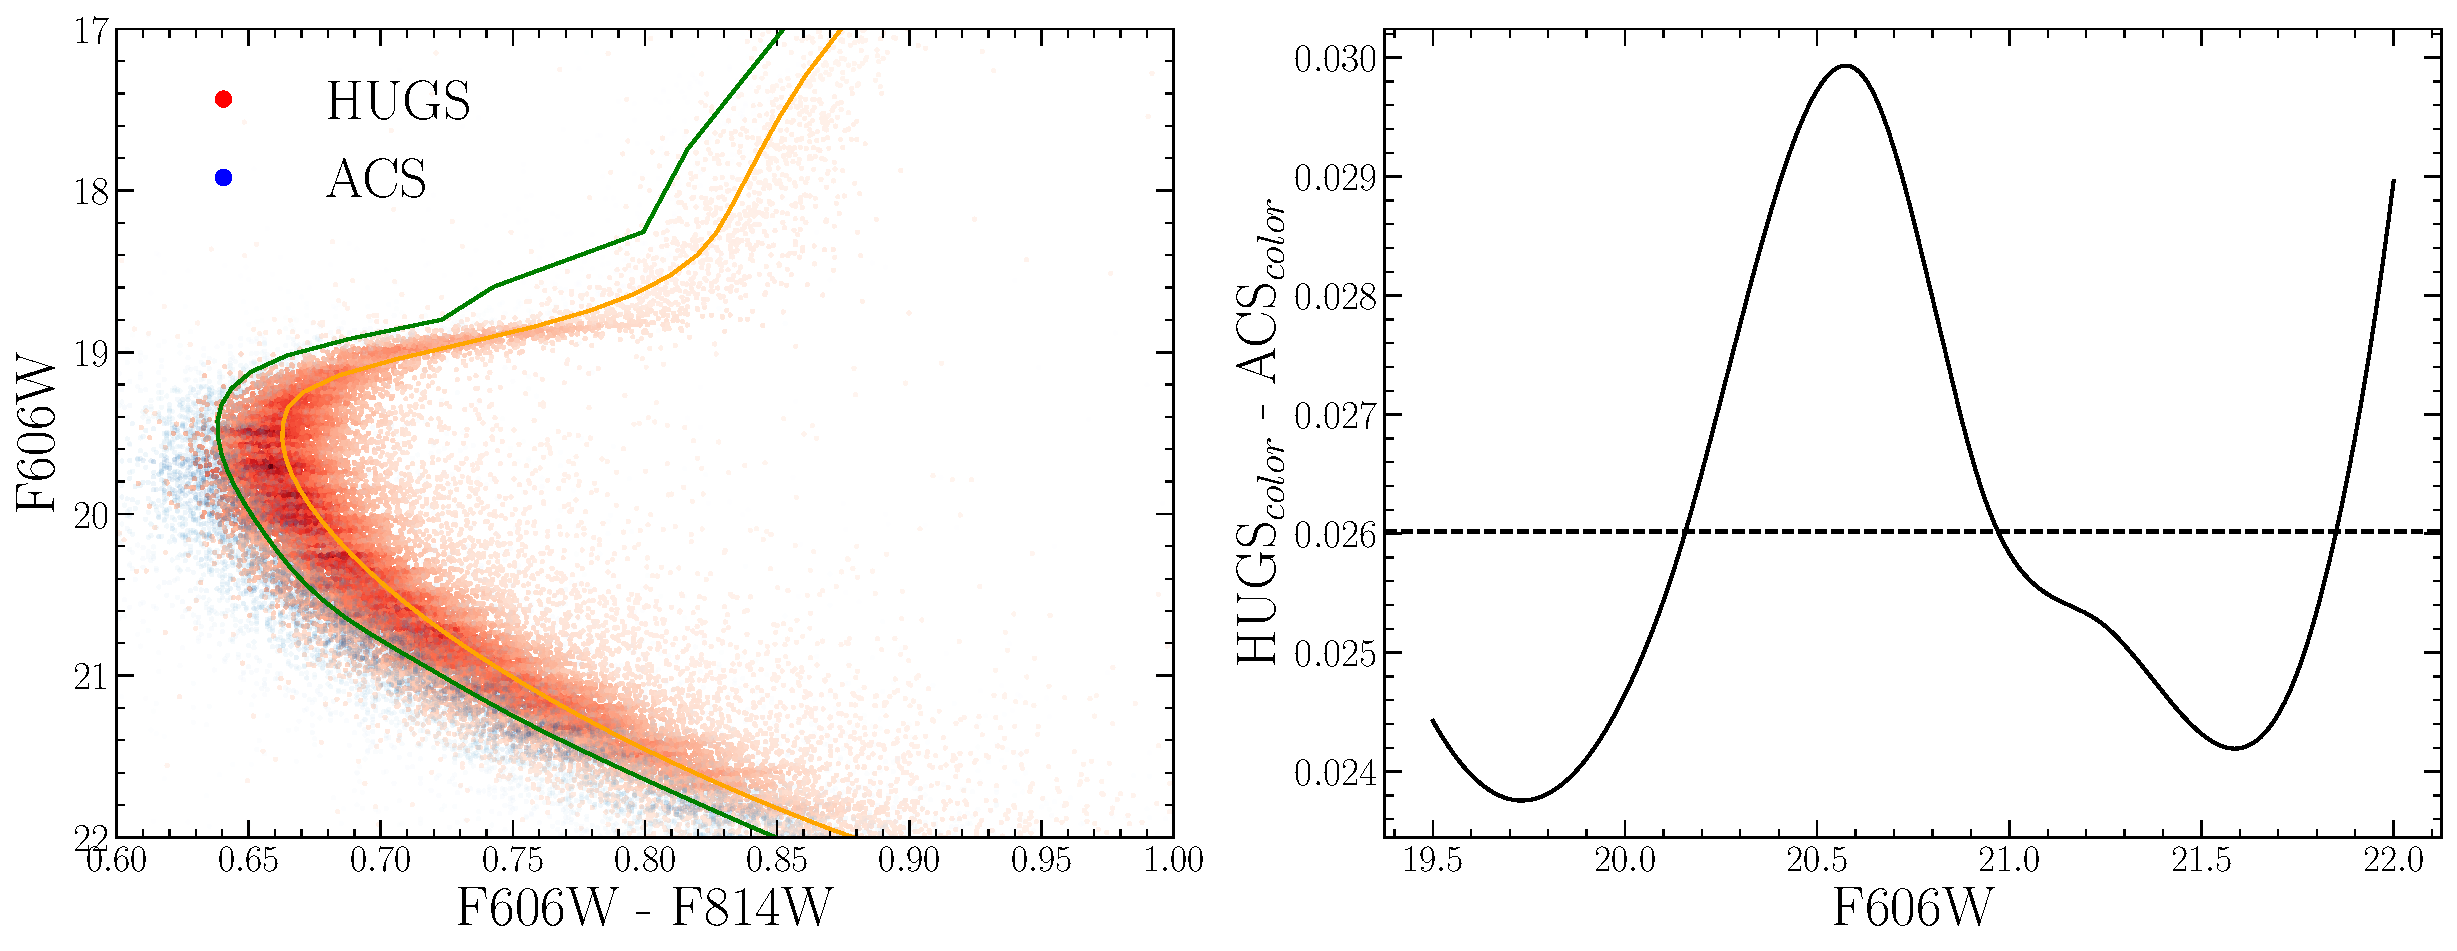
\includegraphics[width=0.90\textwidth]{src/figures/photometricOffset.pdf}
  \label{fig:offset}
  \caption{(left) CMD showing the photometric offset between the ACS and HUGS data for NGC 2808. CMDs have been randomly subsampled and colored by point density for clarity. (right) Mean difference between the color of the HUGS and ACS fiducual lines at the same magnitude. Note that the ACS data is systematically bluer than the HUGS data.}
\end{figure*}

The oberved photometric offset between ACS and HUGS reductions introduces a
systematic uncertainity when comparing parameters derived from isochrone fits
to ACS data vs those fit to HUGS data. Specifically, this offset introduces a
{\color{red}$\sim$AGE Gyr} uncertainity. Moreover, for two isochrone of the
same age, only seperated by helium mass fraction, a shift of the main sequence
turn off of is also expected. Figure \ref{fig:HeMO} shows this shift. Note a change in the helium mass fraction of a model by 0.03 results in an approximate 0.08 magnitude shift to the main sequence turn off location. This means that the mean 0.026 magnitude offset we find in between ACS and HUGS data corresponds to an additional approaximate 0.01 uncertainity in the derived helium mass fraction when comparing between these two datasets. 

\begin{figure}
  \centering
  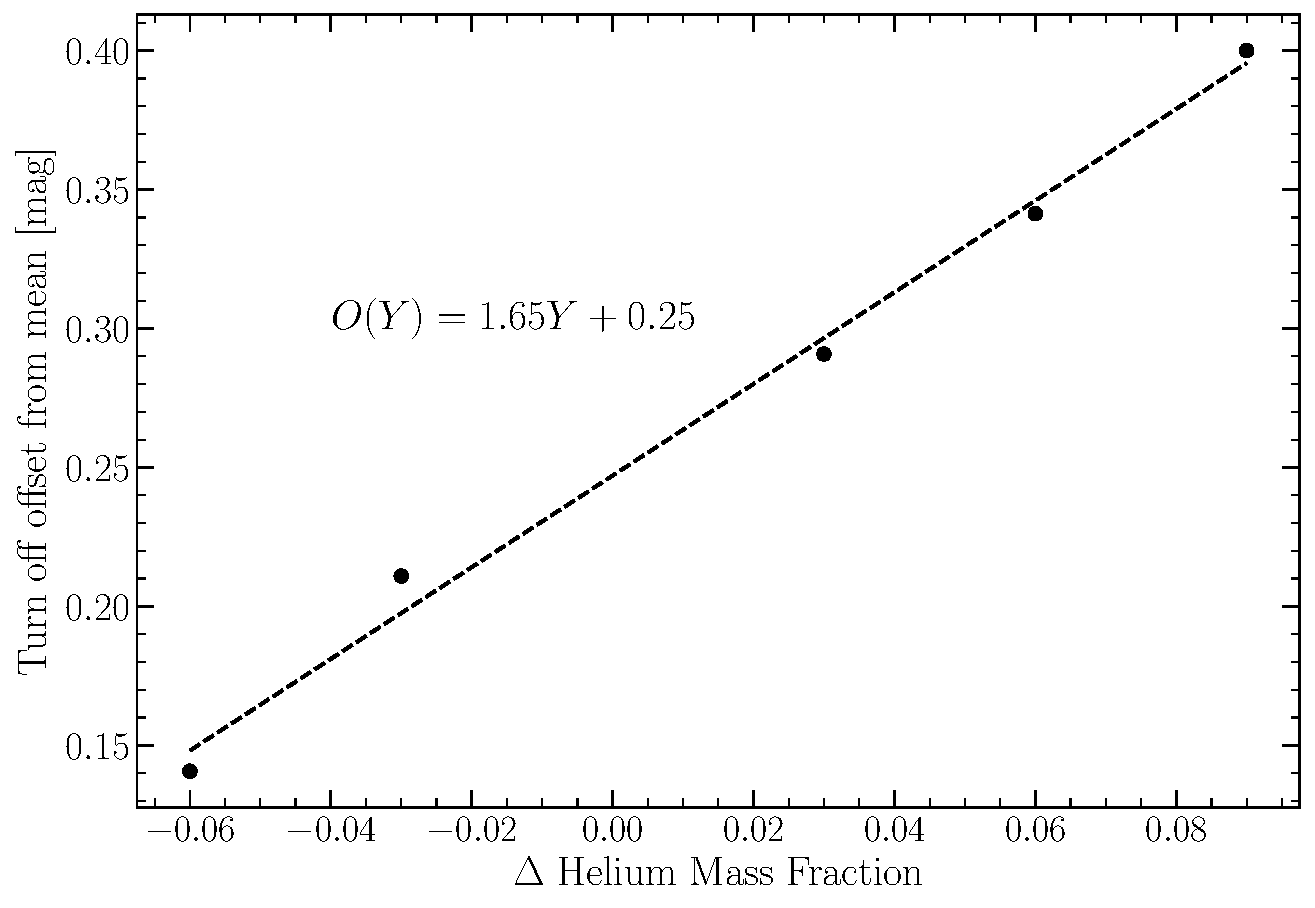
\includegraphics[width=0.45\textwidth]{src/figures/HeliumMeanOffset.pdf}
  \caption{Main sequence turn off magnitude offset from a guage helium mass fraction (Y=0.30 chosen). All main sequence turn off locations are measured at 12.3 Gyr {\color{blue} Should I make these contour surfaces for various ages?}}
  \label{fig:HeMO}
\end{figure}
